\documentclass[a4paper,12pt]{article}

%% Language and font encodings
\usepackage[T1]{fontenc}
\usepackage[polish]{babel}
\usepackage[utf8]{inputenc}
\usepackage{lmodern}
\selectlanguage{polish}

%% Sets page size and margins
%\usepackage[a4paper,top=2cm,bottom=2cm,left=2cm,right=4cm,asymmetric]{geometry}
\usepackage{geometry}


%% Useful packages
\usepackage[fleqn]{amsmath}%[fleqn]
\usepackage{xfrac} %\sfrac{}{}

\usepackage{titlesec}%titles
\titlelabel{\thetitle.\quad}
\let\savenumberline\numberline
\def\numberline#1{\savenumberline{#1.}}
\usepackage{etoolbox}%dots in TOC
\makeatletter
\patchcmd{\l@section}
{\hfil}
{\leaders\hbox{\normalfont$\m@th\mkern \@dotsep mu\hbox{.}\mkern \@dotsep mu$}\hfill}
{}{}
\makeatother

\usepackage{caption,graphicx}
\usepackage{float}
\usepackage{sidecap}
\usepackage[colorinlistoftodos]{todonotes}
\usepackage[colorlinks=true, allcolors=blue]{hyperref}

\usepackage{tikz}
\usepackage{tikz-qtree}
\usetikzlibrary{trees}
\usetikzlibrary{arrows,positioning,shapes,fit,calc,decorations.pathreplacing}
\usetikzlibrary{graphs}
\usetikzlibrary{graphs.standard}
\usepackage{forest}
\usepackage{tikzscale}
\usepackage{pgfgantt} %Diagramy gantta http://bay.uchicago.edu/CTAN/graphics/pgf/contrib/pgfgantt/pgfgantt.pdf
\usepackage{pgf}
\usepackage{caption}

\usepackage{fancybox}
\usepackage{listings}

\usepackage[colorinlistoftodos]{todonotes} %http://mirror.unl.edu/ctan/macros/latex/contrib/todonotes/todonotes.pdf

\usepackage{array,longtable}

\newcommand\floor[1]{\lfloor#1\rfloor} %PODŁOGA -> \floor
\newcommand\ceil[1]{\lceil#1\rceil} %SUFIT -> \ceil

\usepackage{fancyhdr}
\pagestyle{fancy}
\rhead{\thepage}
\lhead{\leftmark}
\rfoot{\thepage}
\lfoot{\rightmark}

%http://tex.stackexchange.com/questions/64170/which-package-to-use-for-writing-algorithms
\usepackage{algorithm}% http://ctan.org/pkg/algorithms
\usepackage{algpseudocode}% http://ctan.org/pkg/algorithmicx
\newcommand{\var}[1]{{\ttfamily#1}}% variable

\algnewcommand\algorithmicforeach{\textbf{for each}} %Algorithm foreach
\algdef{S}[FOR]{ForEach}[1]{\algorithmicforeach\ #1\ \algorithmicdo}

\usepackage{amsthm}
\usepackage[inline]{enumitem} %enumerations
\usepackage{multicol}

\theoremstyle{definition}%~ %%% <-  Note that space!
\newtheorem{lemma}{Lemat} %\begin{lemma} ... \end{lemma} LEMAT(?)
\newtheorem{remark}{Wniosek}%\begin{remark} ... \end{remark} WNIOSEK 
%\newtheorem*{remark*}{Wniosek}%\begin{remark} ... \end{remark} WNIOSEK bez liczby
\newtheorem{theorem}{Twierdzenie}%\begin{theorem} ... \end{theorem}
\newtheorem{fact}{Fakt} %\begin{fact} ... \end{fact}
\newtheorem*{fact*}{Fakt} %\begin{fact*} ... \end{fact*} Fakt
\newtheorem*{observation*}{Obserwacja}

\newtheorem{example}{Przykład}
\newtheorem*{example*}{Przykład} %\begin{example} ... \end{example}
\theoremstyle{definition}
\newtheorem{definition}{Definicja}%\begin{definition}{} ... \end{definition}
%\newtheorem*{definition*}{Definicja}
%\newtheorem*{hipoterm*}{Hipoteza}%\begin{hipoterm*}[] ... \end{hipoterm*}
\newtheorem{hipoterm}{Hipoteza}%\begin{hipoterm*}[] ... \end{hipoterm*}
\theoremstyle{problem}
\newtheorem{problem}{Problem}%\begin{problem}{} ... \end{problem}
\newtheorem*{problem*}{Problem}

\let\originalforall=\forall%FORALL
\renewcommand{\forall}{\mathop{\vcenter{\hbox{\Large$\originalforall$}}}}
\let\originalexists=\exists%EXISTS
\renewcommand{\exists}{\mathop{\vcenter{\hbox{\Large$\originalexists$}}}}

\usepackage{cancel} %skreślenie równania \xcancel{...} \cancel{} lub \bcancel{}

\usepackage{amsfonts}

\usepackage{comment}

\usepackage{xcolor,colortbl}
\usepackage{multirow}

%\usepackage{wrapfig} %wrap text around figure

\usepackage{pdfpages}%\includepdf{file}

\usepackage{etoolbox}
\let\bbordermatrix\bordermatrix
\patchcmd{\bbordermatrix}{8.75}{4.75}{}{}
\patchcmd{\bbordermatrix}{\left(}{\left[}{}{}
\patchcmd{\bbordermatrix}{\right)}{\right]}{}{}
%\bbordermatrix{}

\allowdisplaybreaks

\title{Struktury Dyskretne - Notatki}
\author{Piotr Parysek\\
\href{mailto:piotr.parysek@outlook.com}{piotr.parysek@outlook.com} }
\date{\today}

\begin{document}
\maketitle

\tableofcontents
\section{Ćwiczenia 2: 2-III-2017}
\subsection{Zadania Domowe A}
\paragraph{A1}  Który  z  zamieszczonych  poniżej  rysunków  można narysować  bez  odrywania  ołówka  od  kartki, tak,  że chociaż  przez punkty przecięć linii można przechodzić wielokrotnie,  nie wolno  przesuwać  ołówka  po linii  już narysowanej. Jeśli można to zrobić, wskaż,  w którym punkcie  powinniśmy  zacząć,  a  w  którym  zakończyć rysowanie   linii;   jeśli   nie   jest   to   możliwe   wyjaśnij dlaczego.  Podaj  interpretację  grafową   tego problemu.
\begin{figure}[H]
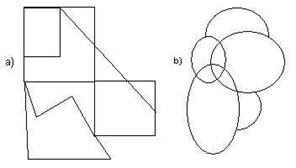
\includegraphics{img/g1}
\end{figure}
\textbf{Odpowiedź:}
\begin{enumerate}[label=\alph*)]
\item Można należy ,,zacząć'' w jednym z nieparzystych punktów przecięć, zakończy się w drugim nieparzystym punkcie. - Szlak Eulera!
\item Nie można - za dużo nieparzystych punktów przecięć.
\end{enumerate}

\paragraph{A2}  Czy poniższe grafy posiadają  cykl Hamiltona?  Jeśli tak, to go wskaż .  Jeśli nie, to uzasadnij dlaczego.
\begin{figure}[H]
\centering
\begin{minipage}{.5\textwidth}
\centering
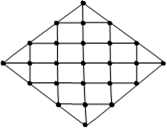
\includegraphics[width=.5\linewidth]{img/g2}
\caption*{a)}
\end{minipage}%
\begin{minipage}{.5\textwidth}
\centering
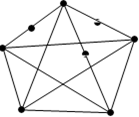
\includegraphics[width=.5\linewidth]{img/g3}
\caption*{b)}
\end{minipage}
\end{figure}

\textbf{Odpowiedź:}
\begin{enumerate}[label=\alph*)]
\item Tak zawiera, nie mam siły przerysowywać ...
\item Jest ścieżka Hamiltona, ale \textbf{Nie wolno} udowadniać Ore albo Dirac, że nie ma lub jest cykl Hamiltona\textbf{!}

Udowodnienie, że nie ma cyklu Hamiltona jest zadaniem z klasy $\mathsf{NP}$- complete
\end{enumerate}

\paragraph{A3}  Czy można obejść szachownicę  $6 \times 6$ koniem szachowym tak, aby każde pole odwiedzić dokładnie raz i wrócić na miejsce startu ?  Jeśli tak – ponumeruj pola zgodnie z trasą  konia; jeżeli nie – uzasadnij dlaczego. \\
\textbf{Odpowiedź:} Tak można:
\begin{table}[H]
\centering
\caption{Szachownica $6\times 6$ z zaznaczoną kolejnością ruchów ,,skoczka''.}
\begin{tabular}{|c|c|c|c|c|c|}\hline
\cellcolor[HTML]{9B9B9B}{\color[HTML]{656565} \textbf{21}} & \textbf{28} & \cellcolor[HTML]{9B9B9B}\textbf{3} & \textbf{26} & \cellcolor[HTML]{9B9B9B}\textbf{19} & \textbf{24} \\\hline
\textbf{2} & \cellcolor[HTML]{9B9B9B}\textbf{11} & \textbf{20} & \cellcolor[HTML]{9B9B9B}\textbf{23} & \textbf{4} & \cellcolor[HTML]{9B9B9B}\textbf{9} \\\hline
\cellcolor[HTML]{9B9B9B}\textbf{29} & \textbf{22} & \cellcolor[HTML]{9B9B9B}\textbf{27} & \textbf{10} & \cellcolor[HTML]{9B9B9B}\textbf{25} & \textbf{18} \\\hline
\textbf{12} & \cellcolor[HTML]{9B9B9B}\textbf{1} & \textbf{14} & \cellcolor[HTML]{9B9B9B}\textbf{33} & \textbf{8} & \cellcolor[HTML]{9B9B9B}\textbf{5} \\\hline
\cellcolor[HTML]{9B9B9B}\textbf{15} & \textbf{30} & \cellcolor[HTML]{9B9B9B}\textbf{35} & \textbf{6} & \cellcolor[HTML]{9B9B9B}\textbf{17} & \textbf{32} \\\hline
\textbf{0} & \cellcolor[HTML]{9B9B9B}\textbf{13} & \textbf{16} & \cellcolor[HTML]{9B9B9B}\textbf{31} & \textbf{34} & \cellcolor[HTML]{9B9B9B}\textbf{7}\\\hline
\end{tabular}
\end{table}

\paragraph{A4}  Przypomnijmy,  że  graf  Eulera  to  taki,  który  ma  obchód  Eulera,  a  graf  Hamiltona  to  taki,  który  ma  cykl Hamiltona.  Czy istnieje graf, który:
\begin{enumerate}[label=\alph*)]
\item ma wszystkie stopnie parzyste, ale nie jest grafem Eulera?\\
\textbf{Odpowiedź:} tak istnieje, na przykład graf nie spójny (ma kilka składowych).

\item jest grafem Eulera, ma nieparzystą  liczbę  wierzchołków i nieparzystą  liczbę  krawędzi ?\\
\textbf{Odpowiedź:} Nie, nie istnieje gdyż zgodnie z twierdzeniem Eulera \ref{the:euler} (na stronie \pageref{the:euler}) graf nie może posiadać wierzchołków stopnia nieparzystego, a gdy posiada nieparzystą liczbę krawędzi to takowe posiada.

\item jest grafem Eulera, ma parzystą liczbę  wierzchołków i nieparzystą  liczbę  krawędzi ?\\
\textbf{Odpowiedź:} %Nie, nie istnieje gdyż zgodnie z twierdzeniem Eulera \ref{the:euler} (na stronie \pageref{the:euler}) graf nie może posiadać wierzchołków stopnia nieparzystego, a gdy posiada nieparzystą liczbę krawędzi to takowe posiada. 
\begin{figure}[H]
\centering
\begin{tikzpicture}[shorten >=1pt, auto, node distance=3cm, ultra thick,main node/.style={circle,draw,minimum size=.4cm,inner sep=0pt]}]%fill=black,
\begin{scope}[every node/.style={font=\sffamily\Large\bfseries}]
\node[main node] (v1) at (0,0) {};
\node[main node] (v2) at (0,1) {};
\node[main node] (v3) at (1,1) {};
\node[main node] (v4) at (1,2) {};
\node[main node] (v5) at (2,2) {};
\node[main node] (v6) at (2,3) {};
\end{scope}
\begin{scope}
\draw  (v1) edge node{} (v2);
\draw  (v1) edge node{} (v3);
\draw  (v2) edge node{} (v3);
\draw  (v3) edge node{} (v4);
\draw  (v3) edge node{} (v5);
\draw  (v4) edge node{} (v6);
\draw  (v5) edge node{} (v6);
%\draw  (v) edge node{} (v);
\end{scope}
\end{tikzpicture}
\caption{Przykład grafu}
\label{fig:zadaniea4c}
\end{figure}

\item jest grafem Eulera, ma parzysta liczbę  wierzchołków, a jego dopełnienie jest grafem Eulera ?\\
\textbf{Odpowiedź:} Nie, nie istnieje, gdyż graf Eulerowski ma wszystkie wierzchołki stopnia parzystego, dopełnienie takiego grafu (przy parzystej liczbie wierzchołków) stworzy graf o nieparzystych stopniach wierzchołków.

\item jest grafem Eulera i grafem Hamiltona, ale nie ma skojarzenia doskonałego?\\
\textbf{Odpowiedź:} przedstawiona na rysunku \ref{fig:zadaniea4e} (na stronie \pageref{fig:zadaniea4e}) graf ma cykl Hamiltona, jest Eulerowski ale nie ma skojarzenia doskonałego. Ogólnie każdy graf o nieparzystej liczbie wierzchołków.
\begin{figure}[H]
\centering
\begin{tikzpicture}[shorten >=1pt, auto, node distance=3cm, ultra thick,main node/.style={circle,draw,minimum size=.4cm,inner sep=0pt]}]%fill=black,
\begin{scope}[every node/.style={font=\sffamily\Large\bfseries}]
\node[main node] (v1) at (0,0) {};
\node[main node] (v2) at (0,1) {};
\node[main node] (v3) at (1,0) {};
\end{scope}
\begin{scope}
\draw  (v1) edge node{} (v2);
\draw  (v1) edge node{} (v3);
\draw  (v2) edge node{} (v3);
\end{scope}
\end{tikzpicture}
\caption{Przykład grafu}
\label{fig:zadaniea4e}
\end{figure}

\item jest grafem Eulera i ma skojarzenie doskonałe, a nie jest grafem Hamiltona?\\
\textbf{Odpowiedź:} przedsawiona na rysunku \ref{fig:zadaniea4f} (na stronie \pageref{fig:zadaniea4f})
\begin{figure}[H]
\centering
\begin{tikzpicture}[shorten >=1pt, auto, node distance=3cm, ultra thick,main node/.style={circle,draw,minimum size=.4cm,inner sep=0pt]}]%fill=black,
\begin{scope}[every node/.style={font=\sffamily\Large\bfseries}]
\node[main node] (v1) at (0,0) {};
\node[main node] (v2) at (0,1) {};
\node[main node] (v3) at (1,0) {};
\node[main node] (v4) at (2,0) {};
\node[main node] (v5) at (0,2) {};
\node[main node] (v6) at (2,2) {};
\node[main node] (v7) at (3,2) {};
\node[main node] (v8) at (3,3) {};
\node[main node] (v9) at (4,2) {};
\node[main node] (v10) at (4,3) {};
\node[main node] (v11) at (5,2) {};
\node[main node] (v12) at (5,3) {};
%\node[main node] (v) at (,) {};
\end{scope}
\begin{scope}
\draw  (v1) edge node{} (v2);
\draw  (v1) edge node{} (v3);
\draw  (v2) edge node{} (v5);
\draw  (v3) edge node{} (v4);
\draw  (v4) edge node{} (v7);
\draw  (v5) edge node{} (v6);
\draw  (v6) edge node{} (v7);
\draw  (v7) edge node{} (v8);
\draw  (v7) edge node{} (v9);
\draw  (v8) edge node{} (v10);
\draw  (v9) edge node{} (v10);
\draw  (v9) edge node{} (v11);
\draw  (v9) edge node{} (v12);
\draw  (v10) edge node{} (v11);
\draw  (v10) edge node{} (v12);
%\draw  (v) edge node{} (v);
\end{scope}
\end{tikzpicture}
\caption{Przykład grafu}
\label{fig:zadaniea4f}
\end{figure}
\begin{proof}
zgodnie z twierdzeniem Dirac'a (\ref{the:Dirac} na stronie \pageref{the:Dirac}):\\ $\delta (G)=2$ a $|V|=12$ wtedy: $\delta (G) \not \geq \frac{|V|}{2}$.
\end{proof}

\item ma skojarzenie doskonałe i cykl Hamiltona, ale nie jest grafem Eulera?\\
\textbf{Odpowiedź:} przedstawiona na rysunku \ref{fig:zadaniea4g} (na stronie \pageref{fig:zadaniea4e}) graf ma cykl Hamiltona, ma skojarzenie doskonałe, ale z powodu, że posiada 2 wierzchołki stopnia nieparzystego nie jest grafem eulerowskim.
\begin{figure}[H]
\centering
\begin{tikzpicture}[shorten >=1pt, auto, node distance=3cm, ultra thick,main node/.style={circle,draw,minimum size=.4cm,inner sep=0pt]}]%fill=black,
\begin{scope}[every node/.style={font=\sffamily\Large\bfseries}]
\node[main node] (v1) at (0,0) {};
\node[main node] (v2) at (0,1) {};
\node[main node] (v3) at (1,0) {};
\node[main node] (v4) at (1,1) {};
\end{scope}
\begin{scope}
\draw  (v1) edge node{} (v2);
\draw  (v1) edge node{} (v3);
\draw  (v2) edge node{} (v3);
\draw  (v2) edge node{} (v4);
\draw  (v3) edge node{} (v4);
\end{scope}
\end{tikzpicture}
\caption{Przykład grafu}
\label{fig:zadaniea4g}
\end{figure}

\item jest dwudzielny, 4-regularny i nie ma cyklu Hamiltona?\\
\textbf{Odpowiedź:} na przykład grad niespójny (na przykład posiadający dwie składowe)

\item jest 10-regularny,  ma 18 wierzchołków i nie ma cyklu Hamiltona?\\
\textbf{Odpowiedź:} wszystkie 18 wierzchołków ma stopień 10 i zgodnie z twierdzeniem Diraca (\ref{the:Dirac} na stronie \pageref{the:Dirac}) i Ore (\ref{the:Ore} na stronie \pageref{the:Ore}) taki graf nie istnieje.

\item jest dwudzielny, 4-regularny i ma cykl Hamiltona, ale nie ma skojarzenia doskonałego?\\
\textbf{Odpowiedź:} Nie - w dwudzielnym grafie regularnym zawsze istnieje skojarzenie doskonałe.
\todo[inline,color=red]{ZADANIE ZAPYTAĆ!}
\item ma parzystą  liczbę  wierzchołków i cykl Hamiltona, ale nie ma skojarzenia doskonałego?\\
\textbf{Odpowiedź:}  
\todo[inline,color=red]{ZADANIE ZAPYTAĆ!}
\end{enumerate}

\paragraph{A5}  Wiadomo, że prawdziwe jest następujące twierdzenie (z wykładu):
Jeśli graf zawiera cykl Hamiltona, to dla dowolnego niepustego podzbioru $S$ zbioru wierzchołków ($S \neq V (G)$) graf $G\setminus S$ ma nie więcej niż $|S|$ składowych.
\begin{enumerate}[label=\alph*)]
\item Czy twierdzenie odwrotne jest prawdziwe ?  Jeśli tak, to uzasadnij; jeśli nie – podaj kontrprzykład.

\textbf{Twierdzenie odwrotne:} Jeżeli dla dowolnego niepustego zbioru $S$ zbioru wierzchołków ($S\neq V(G)$) graf $G\setminus S$ ma nie więcej niż $|S|$ składowych to graf zawiera cyklu Hamiltona.
$$\omega (G\setminus S) \leq |S| \Rightarrow G\rightarrow\text{ zawiera cykl Hamiltona}$$
Nie takie twierdzenie nie jest prawdziwe, na przykład: 
\begin{figure}[H]
\centering
\begin{minipage}{.5\textwidth}
\centering
\begin{tikzpicture}[shorten >=1pt, auto, node distance=3cm, ultra thick,main node/.style={circle,draw,minimum size=.4cm,inner sep=0pt]}]%fill=black,
\begin{scope}[every node/.style={font=\sffamily\Large\bfseries}]
\node[main node] (v1) at (0,0) {1};
\node[main node] (v2) at (1,0) {2};
\node[main node] (v3) at (2,0) {3};
\node[main node] (v4) at (3,0) {4};
\end{scope}
\begin{scope}
\draw  (v1) edge node{} (v2);
\draw  (v2) edge node{} (v3);
\draw  (v3) edge node{} (v4);
\end{scope}
\end{tikzpicture}
\caption*{$G$}
\end{minipage}%
\begin{minipage}{.5\textwidth}
\centering
\begin{tikzpicture}[shorten >=1pt, auto, node distance=3cm, ultra thick,main node/.style={circle,draw,minimum size=.4cm,inner sep=0pt]}]%fill=black,
\begin{scope}[every node/.style={font=\sffamily\Large\bfseries}]
\node[main node] (v1) at (0,0) {1};
\node[main node] (v2) at (1,0) {2};
\node[main node] (v3) at (2,0) {3};
\end{scope}
\begin{scope}
\draw  (v1) edge node{} (v2);
\draw  (v2) edge node{} (v3);
\end{scope}
\end{tikzpicture}
\caption*{$G\setminus S$}
\end{minipage}
\end{figure}
Po usunięciu wierzchołka $S=\{4\}\ $ $\omega (G\setminus S) = 1$, czyli warunek jest spełniony, ale graf $G$ nie jest hamiltoński.

\item Załóżmy,  że  w  pewnym  grafie  $G$,  zawsze  po  usunięciu  dowolnego  zbioru  $S$  wierzchołków  powstaje  graf, który ma nie więcej niż  $|S|$ składowych.  Czy wynika z tego, że $G$ ma cykl Hamiltona?

\textbf{Odpowiedź:} Nie, nie wynika. Aby graf posiadał cykl Hamiltona to musi posiadać cykl i na przykład spełniać warunki twierdzenia Ore lub Diraca. 
\end{enumerate}

\paragraph{A6}  Czy  twierdzenie  odwrotne  do  twierdzenia  Diraca  jest  prawdziwe ?   Jeśli  tak,  to  uzasadnij;  jeśli  nie  – podaj kontrprzykład.

\textbf{Twierdzenie odwrotne:} Jeśli graf $G = (V,E)$ zawiera cykl Hamiltona to $\delta (G) \geq \frac{|V|}{2}$, dla $|V| \geq 3$. \\
\textbf{NIE, NIE JEST PRAWDZIE} 
\begin{figure}[H]
\centering
\begin{tikzpicture}[shorten >=1pt, auto, node distance=3cm, ultra thick,main node/.style={circle,draw,minimum size=.4cm,inner sep=0pt]}]%fill=black,
\begin{scope}[every node/.style={font=\sffamily\Large\bfseries}]
\node[main node] (v1) at (0,0) {1};
\node[main node] (v2) at (0,1) {2};
\node[main node] (v3) at (1,0) {3};
\node[main node] (v4) at (1,1) {4};
\node[main node] (v5) at (2,0) {5};
\node[main node] (v6) at (2,1) {6};
\end{scope}
\begin{scope}
\draw  (v1) edge node{} (v2);
\draw  (v1) edge node{} (v3);
\draw  (v2) edge node{} (v4);
\draw  (v3) edge node{} (v5);
\draw  (v4) edge node{} (v6);
\draw  (v6) edge node{} (v5);
\end{scope}
\end{tikzpicture}
\end{figure}
Graf wyżej nie spełnia warunków, ale jest grafem Hamiltona

\subsection{Zadania Domowe B}
\paragraph{B1} Czy można ułożyć CAR, SAW, SON, HEN, RED, DIM, WIT, HUT, MOB, CUB na cyklu tak, aby
każde dwa kolejne wyrazy miały wspólną literę?
\begin{enumerate}[label=\alph*)]
\item Zinterpretuj problem grafowo.
\item rozwiąż go.
\item W przypadku problemów z rozwiązaniem samodzielnie, skorzystaj z narzędzia: \url{http://users.informatik.uni-halle.de/~jopsi/dass7/}
\end{enumerate}

\textbf{Odpowiedź: }Graf Petersena
\paragraph{B2} Biolog bada bardzo długi łańcuch DNA. Interesuje go, z jakich kolejno nukleotydów składa się łańcuch. Udało mu się z sekwencjonować (odczytać) dużo krótkich fragmentów łańcucha, ponadto wie, że fragmenty te pokrywają cały łańcuch, a niektóre pary się przecinają. Teraz chciałby odtworzyć z nich łańcuch początkowy. Przewidywaną kolejność nukleotydów uważa za prawdopodobną, jeżeli powstaje ona z wszystkich z sekwencjonowanych krótkich łańcuchów, tak kolejno ułożonych, że przynajmniej dwa pierwsze nukleotydy kolejnego łańcucha są ostatnimi w łańcuchu poprzednim. Znajdź co najmniej jeden prawdopodobny długi łańcuch zbudowany z fragmentów (o ile istnieje; mogło się zdarzyć, że biolog zapomniał zapisać jakichś odczytanych sekwencji): TGG, ATTA, GGAA, GGC, TAC, TATT, CATT, GCGG, TACTA, AAAC, TTG, ACA, AACA.
Zinterpretuj problem grafowo dla $n$ z sekwencjonowanych fragmentów.

\textbf{Odpowiedź: }Hamilton, krawędzie skierowane
\paragraph{B3} Narysuj wszystkie parami nieizomorficzne grafy o $6$ wierzchołkach i $6$ krawędziach, które mają obchód Eulera. Proszę jednak nie rysować wszystkich grafów o $6$ wierzchołkach i $6$ krawędziach!

\begin{minipage}{.45\textwidth}
\begin{figure}[H]
\centering
\begin{tikzpicture}[shorten >=1pt, auto, node distance=3cm, ultra thick,main node/.style={circle,draw,minimum size=.4cm,inner sep=0pt]}]%fill=black,
\begin{scope}[every node/.style={font=\sffamily\Large\bfseries}]
\node[main node] (v1) at (0,0) {1};
\node[main node] (v2) at (1,0) {2};
\node[main node] (v3) at (2,1) {3};
\node[main node] (v4) at (1,2) {4};
\node[main node] (v5) at (0,2) {5};
\node[main node] (v6) at (-1,1) {6};
\end{scope}
\begin{scope}
\draw  (v1) edge node{} (v2);
\draw  (v1) edge node{} (v6);
\draw  (v2) edge node{} (v3);
\draw  (v3) edge node{} (v4);
\draw  (v4) edge node{} (v5);
\draw  (v5) edge node{} (v6);
\end{scope}
\end{tikzpicture}
\end{figure}
\end{minipage}%
\begin{minipage}{.45\textwidth}
\begin{figure}[H]
\centering
\begin{tikzpicture}[shorten >=1pt, auto, node distance=3cm, ultra thick,main node/.style={circle,draw,minimum size=.4cm,inner sep=0pt]}]%fill=black,
\begin{scope}[every node/.style={font=\sffamily\Large\bfseries}]
\node[main node] (v1) at (0,0) {1};
\node[main node] (v2) at (2,0) {2};
\node[main node] (v3) at (1,1) {3};
\node[main node] (v4) at (2,2) {4};
\node[main node] (v5) at (0,2) {5};
\node[main node] (v6) at (0,1) {6};
\end{scope}
\begin{scope}
\draw  (v1) edge node{} (v2);
\draw  (v1) edge node{} (v3);
\draw  (v2) edge node{} (v3);
\draw  (v3) edge node{} (v4);
\draw  (v4) edge node{} (v5);
\draw  (v5) edge node{} (v3);
\end{scope}
\end{tikzpicture}
\end{figure}
\end{minipage}
\paragraph{B4} Zbadaj, czy podany graf ma cykl Hamiltona.
\begin{figure}[H]
\centering
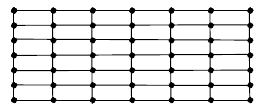
\includegraphics[width=.6\textwidth]{img/2_B4}
\end{figure}

\textbf{Odpowiedź: }Brak
\paragraph{B5} Dla jakich $m, n$ w pełnym grafie dwudzielnym $K_{m,n}$ istnieje:
\begin{enumerate}[label=\alph*)]
\item szlak Eulera ?

\textbf{Odpowiedź: }na przypadki
\item obchód Eulera ?

\textbf{Odpowiedź: }$m,n$ parzyste
\end{enumerate}

\paragraph{B6} Dla jakich $m, n$ w grafie $K_{m,n}$ istnieje:
\begin{enumerate}[label=\alph*)]
\item ścieżka Hamiltona ?

\textbf{Odpowiedź: }$|m-n|=1$
\item cykl Hamiltona ?
\end{enumerate}


\paragraph{B7} Ile różnych cykli Hamiltona jest
\begin{enumerate}[label=\alph*)]
\item w grafie pełnym $K_n$?

\textbf{Odpowiedź: }$\frac{n!}{2n}$
\item w pełnym grafie dwudzielnym $K_{n,n}$?

\textbf{Odpowiedź: }zdrowo rozsądkowo 
\end{enumerate}

\paragraph{B8} Uzasadnij, że jeżeli $G$ ma przynajmniej 2 wierzchołki i $\delta (G) > \frac{V(G) - 1}{2}$, to $G$ zawiera ścieżkę Hamiltona. Wskazówka: można wykorzystać twierdzenie Diraca.

\textbf{Odpowiedź: }
\begin{enumerate}
\item dodanie dodatkowego jednego wierzchołka łącząc z wszystkimi innymi wierzchołkami
\item Dirac
\item jest cykl Hamiltona
\item usunięcie dodanego wierzchołka
\item cykl $\rightarrow$ ścieżka Hamiltona
\end{enumerate}
\paragraph{B9} Na mapie podane zostały miasta wraz informacją, czy możliwe jest i jak kosztowne jest wybudowanie bezpośrednich połączeń między nimi. Zbuduj minimalną, w sensie sumy kosztów, sieć połączeń, która pozwoli na dojechanie (niekoniecznie bezpośrednio) z każdego miasta do każdego. Zinterpretuj problem grafowo i rozwiąż, korzystając z (łatwego do znalezienia w literaturze) algorytmu Prima lub Kruskala.
\begin{figure}[H]
\centering
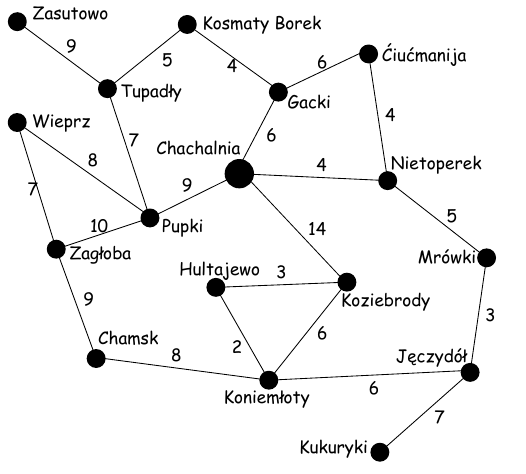
\includegraphics[width=.6\textwidth]{img/2_B9}
\end{figure}

\paragraph{B10} Na rysunku zaznaczono na czerwono pewne drzewo rozpięte w grafie z wagami.
\begin{figure}[H]
\centering
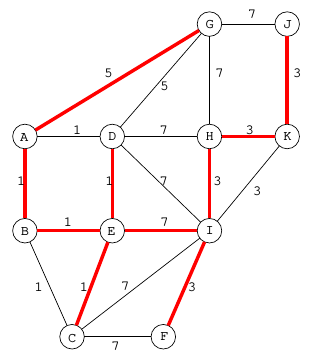
\includegraphics[width=.6\textwidth]{img/2_B10}
\end{figure}
\begin{enumerate}[label=\alph*)]
\item Czy jest to minimalne drzewo rozpięte ?
\item Czy dla tego grafu prawdziwe jest oszacowanie $MST\leq TSP$ ?
\item Czy dla tego grafu prawdziwe jest oszacowanie $TSP\leq 2MST$ ?
\end{enumerate}

\paragraph{B11} Dana jest liczba naturalna $n$. Chcemy ułożyć na okręgu zera i jedynki tak, aby każdy ciąg binarny
długości $n$ wystąpił w tym cyklicznym ciągu jako podciąg złożony z bitów ,,pod rząd” dokładnie raz. Odczytując podciągi, poruszamy się po okręgu zgodnie ze Wskazówkami zegara.
\begin{enumerate}[label=\alph*)]
\item Rozgrzewka: Zinterpretuj problem grafowo. rozwiąż problem dla $n = 3$.
\item Zadanie trudniejsze: rozwiąż problem dla $n = 4$.
\item Zadanie jeszcze trudniejsze: rozwiąż problem dla $n = 5$.
\item Okazuje się (co nie jest oczywiste), że problem ma rozwiązanie dla dowolnego $n$. Zastanów się nad uzasadnieniem tego faktu.
\item Opisz ideę algorytmu znajdującego rozwiązanie dla dowolnego $n$.
\end{enumerate}

\subsection{Zadania}
\paragraph{Zad.1} Zastosuj algorytm Fleury’ego do grafu podanego na rysunku.

\paragraph{Zad.2} Twierdzenie Eulera jest prawdziwe nie tylko dla grafów, ale i dla multigrafów.

Korzystając z tego, uzasadnij poniższe twierdzenie (wniosek z twierdzenia Eulera):
Spójny multigraf ma otwarty szlak Eulera wtedy i tylko wtedy, gdy ma dokładnie dwa wierzchołki nieparzystego stopnia.

\paragraph{Zad.3} Czy można obejść szachownicę $5\times 5$ koniem szachowym tak, aby każde pole odwiedzić dokładnie raz i wrócić na miejsce startu ? Jeśli tak – ponumeruj pola zgodnie z trasąkonia; jeżeli nie – uzasadnij dlaczego.

\paragraph{Zad.4} Zbadaj, czy dany graf ma cykl Hamiltona.

\paragraph{Zad.5} Czy istnieje graf, który:
\begin{enumerate}[label=\alph*)]
\item jest grafem Eulera, ma parzystą liczbę wierzchołków i nieparzystą liczbę krawędzi, który w dodatku jest regularny ?
\item jest dwudzielny, 4-regularny i nie ma obchodu Eulera?
\item ma taki ciąg stopni wierzchołków: (6,6,5,5,4,4,4,4) ale nie ma skojarzenia doskonałego?
\end{enumerate}

\paragraph{Zad.6} Czy k-kostka $Q_k$ jest grafem Eulera?

\paragraph{Zad.7} Ile różnych cykli Hamiltona jest w grafie $K_n$ ?

\paragraph{Zad.8} Czy k-kostka $Q_k$ zawiera cykl Hamiltona? Zadania do samodzielnego rozwiązania później (najlepiej przed kolokwium)


%--------------------------------------------------
\end{document}
